\chapter{\IfLanguageName{dutch}{Stand van zaken}{State of the art}}
\label{ch:stand-van-zaken}

% Tip: Begin elk hoofdstuk met een paragraaf inleiding die beschrijft hoe
% dit hoofdstuk past binnen het geheel van de bachelorproef. Geef in het
% bijzonder aan wat de link is met het vorige en volgende hoofdstuk.

% Pas na deze inleidende paragraaf komt de eerste sectiehoofding.

Dit hoofdstuk bevat je literatuurstudie. In dit onderdeel zal er diep in gegaan worden op het onderwerp. Delen van het onderwerp worden grondig onderzocht om later tot een conclusie te komen. 

\section{Microservices}
\subsection{Definitie}
Een term die vaak zal terug keren in deze paper is 'monolithic'. Deze term betekend het volgende: Bij een monolithic communiceren alle deeltjes van een applicatie met een grote databank of datastore. In een databank of datastore wordt er info en data opgeslaan om dit dan later te gebruiken. De data kan later gebruikt worden om het gepasseerde semester van een bedrijf te analyseren. 
Het artikel van \textcite{Mauersberger2017} geeft meer uitleg over microservices door de moeilijkheden bij een monolithic aan te kaarten. Bij een verandering binnen een monolithic architectuur, wordt er een heel nieuwe versie van de architectuur uitgebracht. Een verandering brengt een hoop extra werk mee. Dit omvat 
\begin{itemize}
	\item De volledige architectuur moet opnieuw getest worden.
	\item Deze architectuur kan heel complex worden bij het groter worden en toevoegen van functionaliteiten.
	\item De complete architectuur moet opnieuw gedeployed worden bij elke update.
	\item De impact van een verandering kan verkeerd ingeschat worden.
	\item Bij een fout in een proces, kan de volledige architectuur falen.
\end{itemize}
De definitie die te vinden is in dit artikel, gaat als volgt: "A method of developing software applications as a suite of independently deployable, small, modular services in which each service runs a unique process and communicates through a well-defined, lightweight mechanism to serve a business goals.". Als je de definitie leest, zie je drie onderdelen. Het eerste onderdeel vertelt hoe een microservice in elkaar zit. Het is een onafhankelijke, kleine, modulaire services. Modulaire services zijn services waarbij veel delen uitwisselbaar zijn met diverse services. De services staan los van elkaar. Ze hebben geen invloed op elkaar. Daarom zijn ze ook onafhankelijk. Wordt er info gestuurd of gevraagd van services A dan zal dit geen invloed hebben op de andere services. De eenvoudige communicatie is een tweede eigenschap van microservices. Er is nood aan communicatie omdat sommige services wel data moeten uitwisselen om hun 'job' te kunnen doen. De communicatie kan gebeuren op verschillende manier. De manier die gekender is, is 'Messaging via a Message Broker'. Dit wil zeggen dat microservice A een bericht plaats op de wachtrij bij microservice B wanneer die data wil doorsturen. Dan Kan microservices B aan die data wanneer hij die nodig heeft. Ze zullen soms moeten wachten op elkaar maar ze zijn zo goed als onafhankelijk van elkaar. De derde eigenschap omvat dat een microservice wordt gemaakt in functie van een requirement uit de business. Elk product in de business heeft een doel dat moet voldoen aan eisen. Het unieke aan microservices is dat we ze gaan bekijken vanuit de eisen binnen de business. Het doel van microservices is, de problemen die te vinden zijn bij een monolithic, verhelpen. De vorige definite legde uit wat microservices zijn. Dit artikel zegt waar men microservices kan plaatsen. Er is dus één groot framework. Daar zitten meerdere onafhankelijke services in.
\begin{figure}[h]
	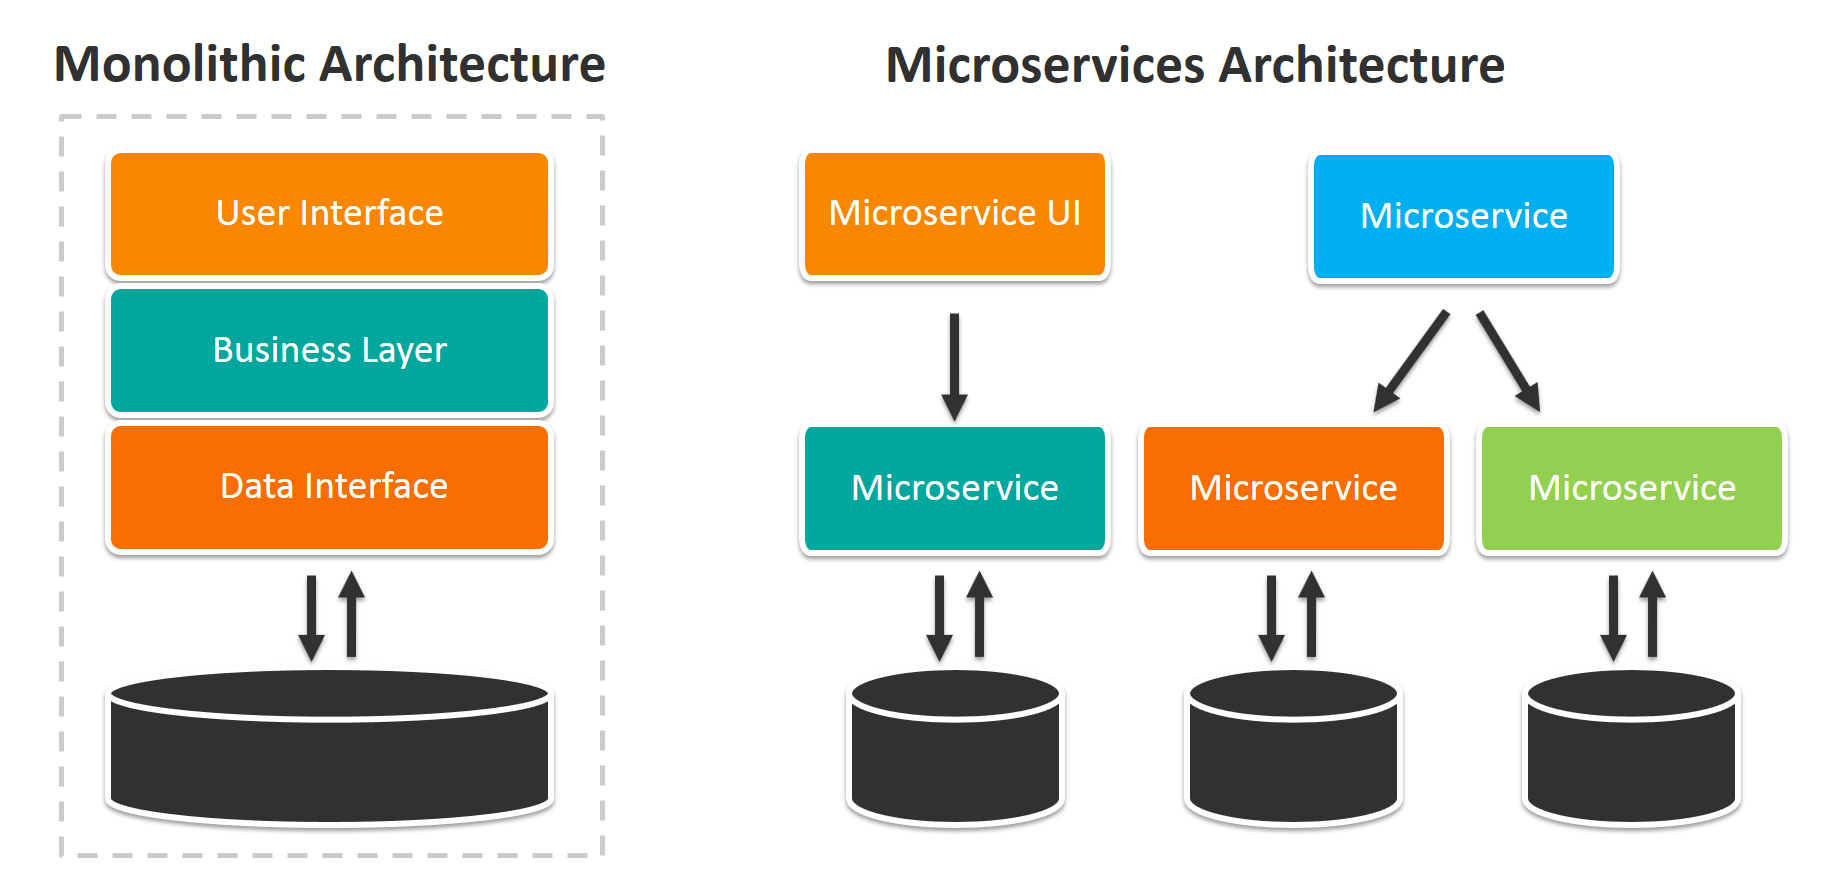
\includegraphics[width=10cm]{microservices-vs-monolithic.jpg}
	\centering
	\caption{Een monolithic architectuur naast een microservice architectuur. \textcite{Watts2018}}
\end{figure}
Figuur 2.1 is afkomstig uit artikel \textcite{Watts2018}.
Zoals te zien in figuur 2.1 is er een groot verschil tussen een monolithic architectuur en die van een microservice. De monolithic wordt weergegeven in de linkerkant van de foto. Aan de rechterkant van de foto is een voorbeeld te zien van een microservice architectuur. Daar is duidelijk te zien dat elke microservice een eigen databank/datastore heeft. Voor elke functionaliteit wordt een microserives aangemaakt, die dan nog eens apart een databank voor zich krijgt. Als bij microservice A een probleem is dan heeft dit niet meteen impact op de andere services. De communicatie tussen microservice A en de anderen zal wel hinder ondervinden. Maar de andere microservices kunnen wel nog steeds onafhankelijk verder. 
Het artikel van \textcite{series2018} bestaat uit elf verschillende onderdelen. Eerst wordt er uitleg gegeven over wat microservices zijn. Dit is hun definitie van microservices: "A software architecting pattern that allows software to be developed into relatively small, distinct components. Each of the components is abstracted by an API(s) and provides a distinct subset of the functionality of the entire application". Ook hier zien we weer het puntje passeren dat een microservice een klein componentje is van een groter geheel. Die eigenschap wordt heel hard benadrukt. Na het uitleggen van microservices, schrijven ze ook over hoe microservices zo scalable zijn. Met scalable bedoelen ze schaalbaarheid. De mogelijkheid van software om mee te groeien als het aantal gebruikers vermeerderd. Dus eigenlijk dat de software nog steeds even goed presteerd bij 10 gebruikers als bij 2 000 gebruikers. Ook lichten ze toe hoe belangrijk API's zijn binnen een microservice architectuur. API's zijn een set van definities die ervoor zorgen dat deeltjes in een programma met elkaar kunnen communcieren. Een voordeel van API's is dat je niet moet weten hoe de andere code werkt. Verder wordt er ook gepraat over de verschillen tussen een monolithic architectuur en een microservice architectuur. 
\subsection{Het belang van microservices}
Bij een monolithic kan het aanpassen van een deeltje, veel werk vragen. Dit werd meer uitgelegd bij de definite van microservices. Microservices spelen gemakkelijker in op het periodieke opleveren van delen software. Deze technologie legt niet heel het framework plat als er deeltjes moeten bij gecodeerd worden. Microservices kunnen sneller inspelen op de Agile analyse/ontwikkel methode. Dit is ook een reden waarom microservices zo een opkomst kent. De analyse methode Agile werkt met periodieke opleveringen die kunnen gaan van twee weken tot een maand. In de periode wordt er gewerkt aan een functionaliteit of een eis van de klant. 
\textcite{series2018} haalt aan dat microservices van belang zijn bij het scalen van software.
In het artikel van \textcite{RDX2016} worden er verschillende eigenschappen aangekaart. Microservices moeten een doel in de business vervullen. Naast dit, zorgt microservices er ook voor dat bescherming eenvoudig wordt. 
Zoals te vinden is in het artikel van \textcite{Troisi2019} zijn er acht manieren hoe microservices bescherming bieden. NOG VERDER UITSCHRIJVEN.
Het artikel van \textcite{Watts2018} geeft het belang van een microservice goed weer. Microservices beschermen het gehele systeem, bij een goede implementatie. Het toepassen van de agile methode is eenvoudiger bij microservices dan bij een monolithic. Met deze technologie is het eenvoudiger om een aanpassing te testen en te onderhouden. Niet de volledige architectuur moet opnieuw getest worden bij een aanpassing. Als team A een aanpassing doet aan hun microservice, zullen de andere teams geen hinder ondervinden. 
\subsection{Algemene aanpak om microservices te implementeren}
Het interessante artikel van \textcite{Benetis2016} over een 6-stappen plan om microservices te implementeren. Een paar woorden die meer verklaring nodig hebben voordat we verder gaan. Een gateway is een netwerkpunt dat dient als toegang tot een ander netwerk. Een gateway is een soort toegangspoort. Implementatie is een procesmatige invoering van een verandering of vernieuwing. Iets implementeren of vernieuwen. 
--------------------- Nieuw
In grote lijnen is dit het zes-stappen plan. Als eerste komt aan bod "serve a business purpose". Hierna komt "protect your stuff". Eens dat gebeurt is, zegt het artikel "see no evil, hear no evil". Dan komt "find your stuff" aan bod. Hierna wordt de volgende stap "create a gateway" aangehaald. Als laatste komt "construct events" aan de beurt. 
Bij eerste stap, "Serve a business purpose", zegt de titel al veel van wat er verwacht wordt. Een microservices is gebaseerd op een business requirement. En niet het doel dat het IT-team voor ogen heeft. Een voorbeeld van een business requirement is het ophalen van data om die dan te analyseren om daar later dan conclusies uit te trekken. Dit kan in een microservices gegoten worden. Eens het doel voor ogen is bij een microservices, moet er ook gekeken worden naar wat de microservices moet kunnen. Zo lang het bij enkele microservices blijft, is automated deployement etc. niet zo belangrijk. Maar eens we gaan scalen en meerdere microservices in één systeem steken zouden volgende puntjes toch self-sufficient moeten zijn:
\begin{itemize}
	\item Geautomatiseerde implementatie
	\item Blootstelling aan andere systemen, toegankelijk eindpunt
	\item Opslag van data
	\item Schaalbaarheid en belasting
\end{itemize}
Zoals te zien is op figuur 2.3, is een microservices één klein deeltje in een groot geheel. Later in dit stappenplan zal de figuur ook uitgebreidt worden en zal het geheel duidelijk worden. 
\begin{figure}[h]
	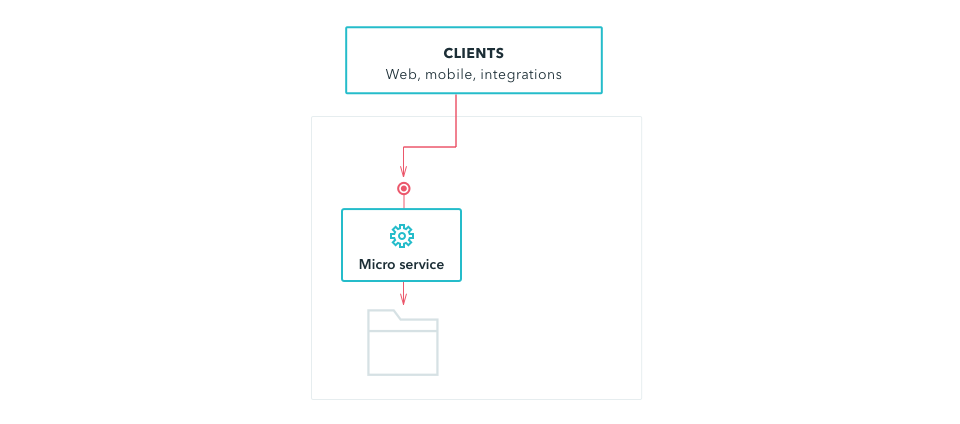
\includegraphics[width=10cm]{1.png}
	\caption{Een microservice dat voldoet aan een business requirement. \textcite{Benetis2016}}
	\centering
\end{figure}

Na "Serve a business purpose" komt "Protect your stuff". Dit gaat over de bescherming van een microservices. Als het gaat over bescherming moet dit op elk moment gebeuren. Ookal heb je maar één à twee microservices, of honderden, bescherming is belangrijk. Het is belangrijk op over al de microservices een uniforme manier te vinden om ze te beschermen. De bescherming kan een requirement op zich zijn, dus ook dit kan in een microservices worden gestoken. Bescherming is een vage term daarom een korte uitleg van hoe een bescherming er zou kunnen uitzien. De meest bekende manier is natuurlijk authorisatie en authenticatie. Authorisatie is het verkrijgen van rechten om bijvoorbeeld een product toe te voegen op een site. Authenticatie is het aanmelden op facebook bijvoorbeeld. De controle of jij het wel echt bent. Een manier op de microservices te beschermen is gecentraliseerde session opslag. Hier zal verder in de thesis nog dieper op worden ingegaan. Kort uitgelegd betekend gecnetraliseerde session opslag dat de data van de user centraal opgeslagen staat. Zodat alle microservices de zelfde session data lezen en gebruiken. 
\begin{figure}[h]
	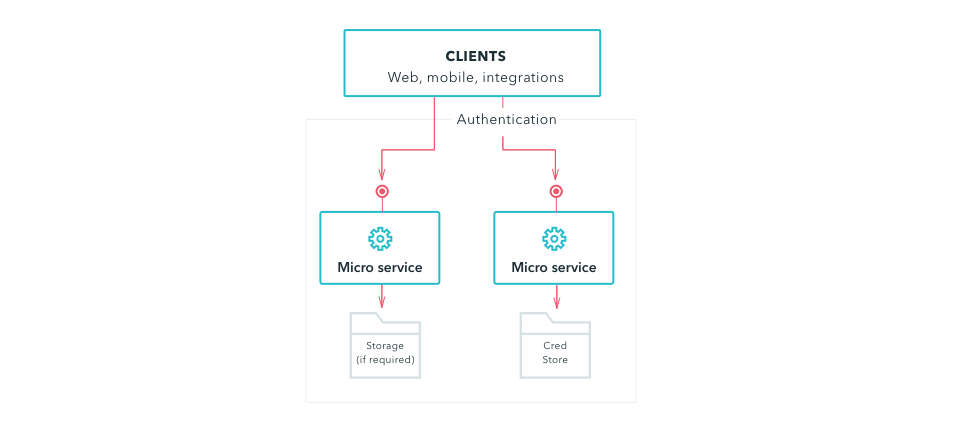
\includegraphics[width=10cm]{2.png}
	\caption{Een microservice waar bescherming aan is toegevoegd. \textcite{Benetis2016}}
	\centering
\end{figure}
In figuur 2.4 is de authenticatie in een microservices gestoken. 

Na de eerste twee stappen komt "See no evil, hear no evil". Eens de microservice is opgezet en gedeployed, moet er gemonitord worden. Daarmee wordt bedoeld dat hoe de microserivces zich gedraagd goed moet bijgehouden worden. Alles zou goed moeten gelogd worden, zodat bij een probleem het geen moeite is om te vinden waar het probleem zich voordeed. Ook hier is het aangeraden om doorheen het hele systeem een uniforme manier van loggen aan te houden. Ook kan men hiervan een microservice maken. Dit wordt ook afgebeeld in figuur 2.5.
\begin{figure}[h]
	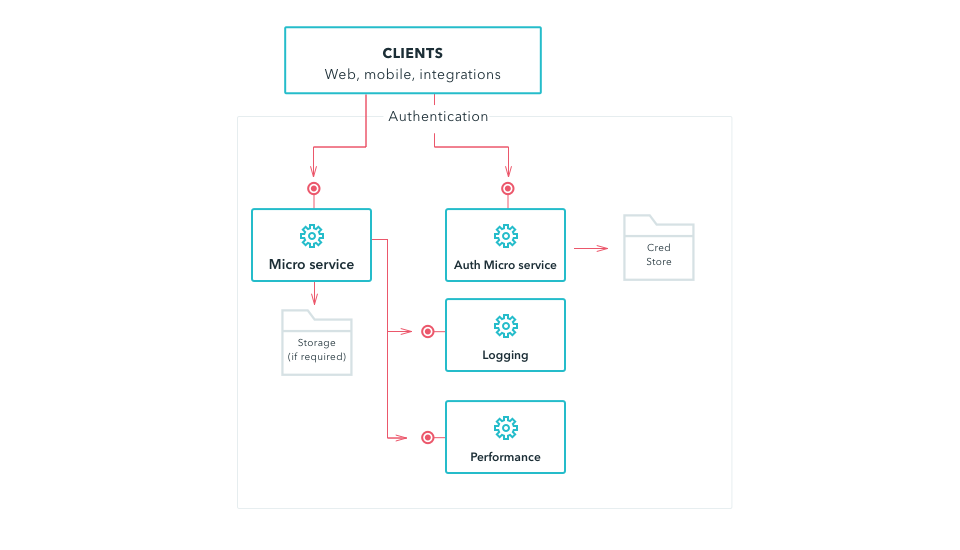
\includegraphics[width=10cm]{3.png}
	\caption{Een microservice waar er monitoring is aan toegevoegd om chaos te voorkomen. \textcite{Benetis2016}}
	\centering
\end{figure}


---------------------oud

\begin{figure}[h]
	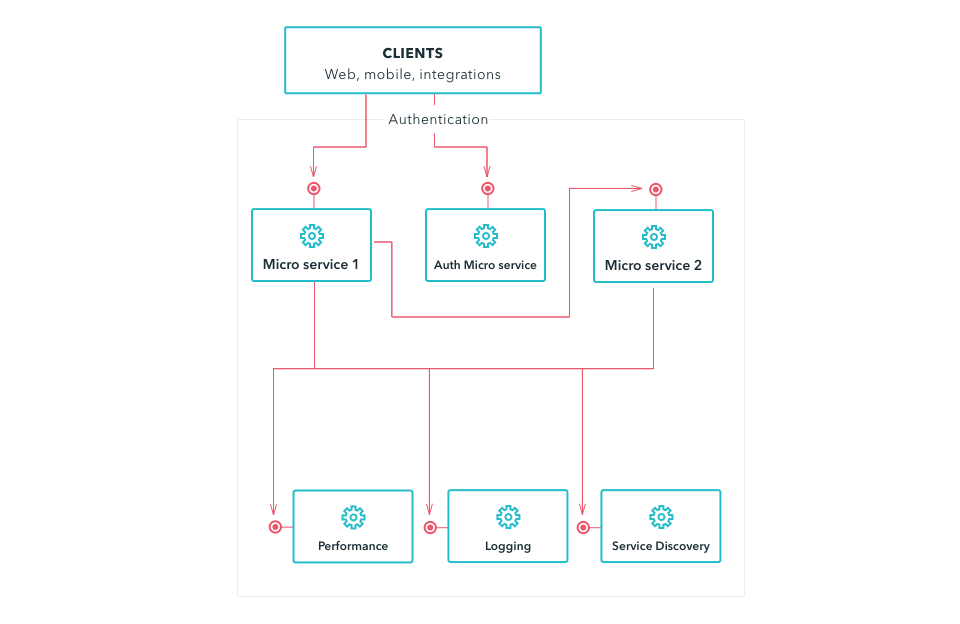
\includegraphics[width=10cm]{4.png}
	\caption{Een microservice dat authenticatie als bescherming toepast. \textcite{Benetis2016}}
	\centering
\end{figure}
Als tip wordt er gegeven om abstractie te gebruiken. Dit is mogelijk door een microservice of compononent te creëeren. Na dat dit allemaal opstaat, is er nog iets waar men nood aan heeft. Een gateway gebruiken. Dit zorgt ervoor dat je implementatie 'weggestopt' zit. Een API gateway is een microservice. Deze zorgt ervoor dat de klant de juiste microservice te pakken krijgt. Je kan het zien als een soort winkelbediende die je helpt bij het vinden van een broek. Een opsomming welke functies een API gateway kan hebben:
\begin{itemize}
	\item Beveiliging van je architectuur,
	\item de prestatie van alle aanvragen kunnen geregistreerd worden,
	\item auditing, 
	\item het transformeren van een of meerdere request naar een microservice,
	\item het implementeren van dynamische requests en routing.
\end{itemize}
Hoe een gateway kan gebruikt worden bij microservices, is te zien op figuur 2.6.
\begin{figure}[h]
	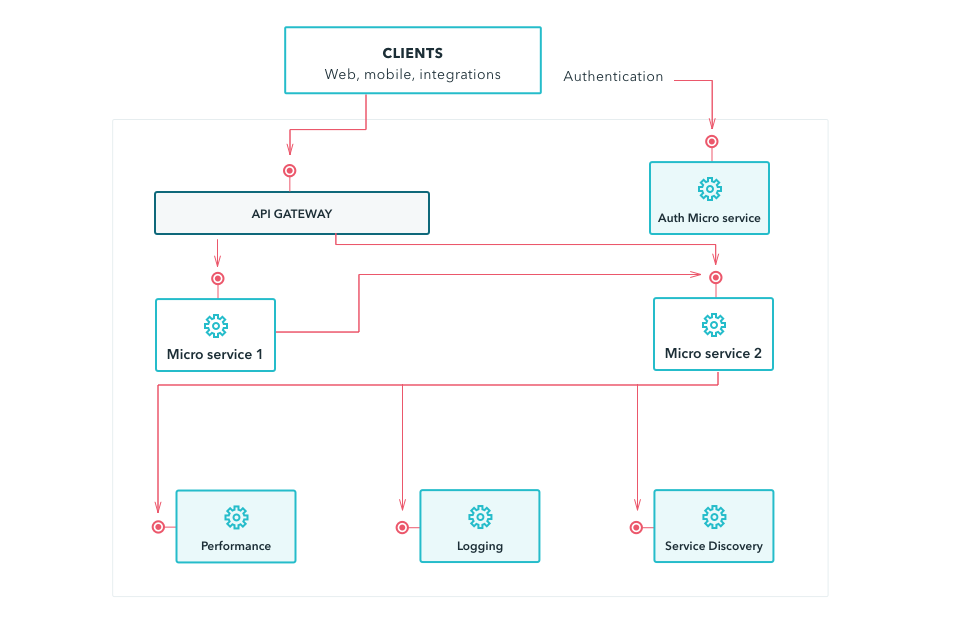
\includegraphics[width=10cm]{5.png}
	\caption{Een microservice dat een gateway gebruikt. \textcite{Benetis2016}}
	\centering
\end{figure}
Als laatste puntje komt de asynchroniteit aan bod. Message queues zijn een oplossing. Om dit aan te pakken, kan je een microservice maken die voor deze taak zorgt. Op deze manier kan je:
\begin{itemize}
	\item Taken inplannen,
	\item subscriben voor specifieke events,
	\item je subscribe functie laten 'zien' aan externe klanten om notificaties aan te kunnen.
\end{itemize}
In figuur 2.7 is het eindresultaat te zien van alle zes de puntjes.
\begin{figure}[h]
	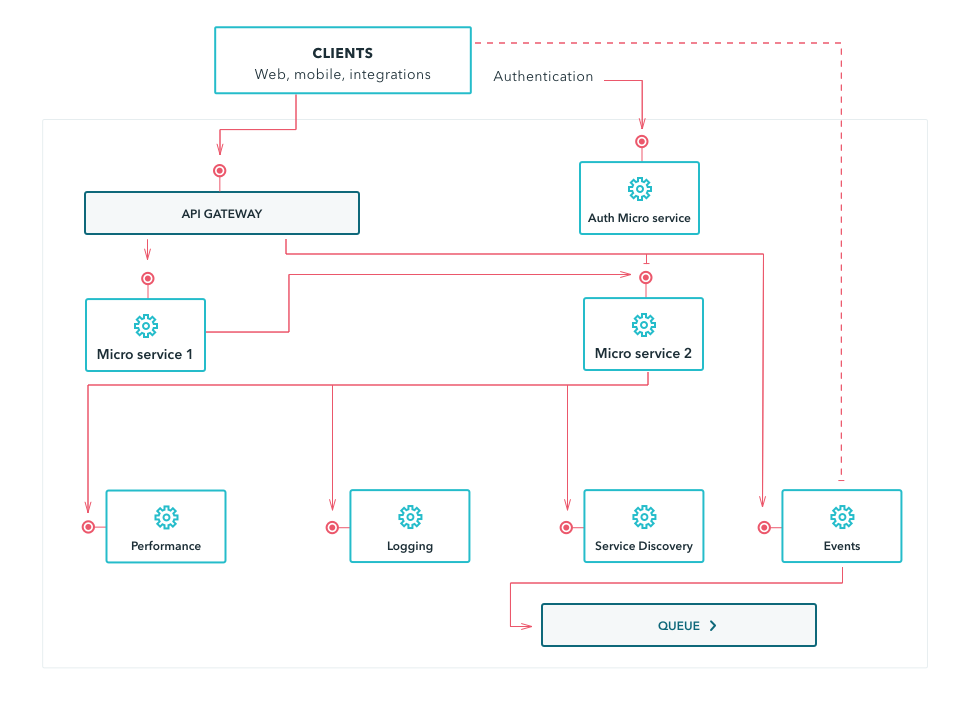
\includegraphics[width=10cm]{6.png}
	\caption{Een microservice met asynchronisatie. \textcite{Benetis2016}}
	\centering
\end{figure}


\subsection{De voordelen en nadelen van microserivces}
In het artikel van \textcite{series2018} wordt er veel lofzang gedaan over microservices. Het gebruik van microservices zou ervoor zorgen dat de architectuur flexibeler wordt. Met flexibeler wordt bedoelt dat de architectuur zich kan 'aanpassen' of kan inspelen op verschillende situaties. Er kunnen microservices hergebruikt worden. Dankzij microservices is het hermodeleren, implementeren van nieuwe technologieën, ... 
Kleinere deeltjes zijn gemakkelijker te documenteren. De snelheid van microservices zijn een groot pluspunt. Hiermee wordt er geprobeert om aan te halen dat microservices sneller reageren omdat zo kleine, onafhankelijke services zijn. Ze moeten geen 'onnodige' stappen maken om de wens van de klant te vervullen. 
\textcite{Watts2018} geeft enkele voordelen van een microservice. Een developer is onafhankelijk. Ze hebben vrijheid. Ook het scalen van een microservice is veel eenvoudiger. Dit komt door dat microservices minder resources nodig hebben dan een volledige monolithic. Resources zijn hulpbronnen. Zoals al vaak aangehaald in deze bachelorproef, zijn microservices onafhankelijk en zouden ze daarom ook geen hulpbronnen nodig mogen hebben. Binnen een monolithic zijn deeltjes afhankelijk van elkaar en hebben elkaar dus nodig om goed te kunnen functioneren. De deeltjes binnen de monolithic hebben elkaar dus nodig en mogelijk als hulpbron. Een ander voordeel is bij het falen van een microservices, de andere microservices er geen last van zullen hebben. Dit komt door hun onafhankelijkheid. 
\subsection{Voorbeelden}
In dit deeltje zal je meer te weten komen over hoe grote technologische bedrijven microservices toepassen en hoe ze naar deze technologie zijn overgeschakeld.
Een term die hier vaak zal gebruikt worden, is een monolithic. Dit is de tegenhanger van microservices. Sommige zweren bij monolithic en anderen hebben gouden woorden voor microservices. De beslissing om één van de twee technieken te kiezen, ligt bij wat je precies nodig hebt. Wat de business nodig heeft. 

\subsubsection{Amazon}
\textcite{Mauersberger2017} gaf een voorbeeld waarom Amazon overstapte. Zoals veel grote bedrijven is Amazon begonnen met een grote monolithic. Een van de nadelen die Amazon ondervond aan deze technologie is de moeilijkheid van het inschatten van de zwaarte op de servers. Daardoor verloor Amazon veel geld en was er nood aan herstructurering.
\textcite{Fulton2015} legt ook uit waarom Amazon is overgeschakeld. Het blijkt dat Amazon in 2001 de grootste monolithic was in de retail business. Doordat Amazon een snel groeiende onderneming was, werd de monolithic architectuur heel ingewikkeld. Amazon hun aanpak was, gooi wat je hebt niet weg maar maak het eenvoudiger. 
\subsubsection{Apple}
\subsubsection{Facebook}
\subsubsection{Netflix}

\section{Order-to-cash proces in SAP}
\subsection{Definite}
\textcite{Obrien2017} geeft aan dat een order-to-cash bestaat uit processen met business requirements. Dit proces start bij het plaatsen van een order en eindigt bij het innen van het geld. Het proces is in de grote lijnen hetzelfde. Het snel doornemen van het proces, geeft een vertekend beeld. Elk deeltje van dit proces heeft moeilijkheden en uitdagingen. 
Dit proces is heel belangrijk voor bedrijven. Het is de core van de business. Bij een slechte implementatie, kan je klanten verliezen of geld verliezen. 
\subsection{Technologie}
\subsubsection{Onderdelen van een order-to-cash proces}
Er zijn vier grote onderdelen, namelijk:
\begin{itemize}
	\item Voor-verkoopsactiviteiten.
	\item Het order proces.
	\item Order afwerking.
	\item Betaling.
\end{itemize}
Bij de voor-verkoopsactiviteiten verstaan we het contact dat moet worden gemaakt worden met klant. De klant moet overtuigd worden van het product. Na contact komt er al dan niet een offerte. Soms kan er ook van contact rechtstreeks naar een order gaan. 
Het orderproces bevat maar één onderdeel namelijk: de sales order. 
Binnen de order afwerking valt het leveren van goederen, het verzenden van goederen.
\textcite{Kumaran2015} geeft een mooi overzicht van de stappen die een order to cash proces kan bevatten. Zo begint het artikel met een toelichting dat dit proces een core proces is van de business. Dit wil zeggen dat een bedrijf, zonder dit proces, geen winst kan maken. Het is een essentieel onderdeel van zo wat elk bedrijf. Hoe deze vorm krijgt binnen een bedrijf, is heel verschillend. Een OTC proces start met het ontvangen van orders. Daarna kan, dit gebeurt niet overal, er gekeken worden naar het krediet van de klanten. Mag deze klant wel nog een bestelling plaatsen? Hierna wordt het order opgenomen in het systeem. Het product wordt verzonden en geleverd. En als laatste wordt de factuur betaald. Dit is welliswaar het 'perfecte' verloop van een order to cash proces. 
\begin{figure}[h]
	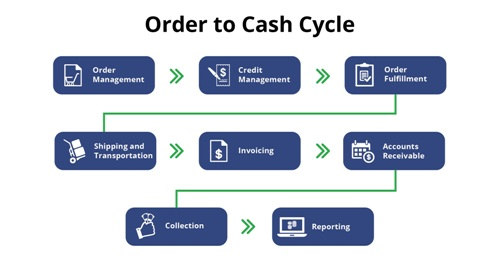
\includegraphics[width=10cm]{Order-to-cash-cycle.jpg}
	\caption{Order-to-cash proces volgens \textcite{Kumaran2015}.}
	\centering
\end{figure}
Er zijn ook enkele uitdagingen verbonden met dit proces. In de volgende opsomming vindt je er enkele:
\begin{itemize}
	\item Hou de orders goed bij, anders loopt het fout vanaf het begin. 
	\item Zonder automatisering verlies je veel tijd. Kostbare tijd.
	\item Zorgen dat de logistiek 'on point' is, is heel belangrijk. Dit is een belangrijk onderdeel binnen het proces.
	\item Bij wanbetalingen, moet de customer service ingrijpen. Ook zij zijn een belangrijk onderdeel van het proces.
\end{itemize}
Het managen van een OTC proces is even belangrijk als de andere aspecten. Een slecht gemanaged proces kan op lange termijn duurder uitkomen dan een onderdeel dat nog niet geautomatiseerd is. 
\subsubsection{Wat biedt SAP zelf aan voor microservices}
\subsection{Een order-to-cash proces vanuit de business}
\subsection{Het proces afstemmen met de business}

\section{Requirements van de business}

